From the use cases listed in figure \ref{tab:actoreventtable} only some is sophisticated enough to be described in detail.  
The use cases add tag, delete tag, add category, delete category, administrate staff, administrate department, and \gstat[] will be omitted, since they are trivial and/or backend administration. 

\paragraph{See all problems} The use case see all problem is used by both \aclient{} and \astaff{} and works as a searchable list. 

\paragraph{\bloadwork[c]} \bloadwork[c] is the operation of the \wmon{} it checks and compares all staff members workload and redistribute problems in order to equally balance the workload in each department. 

\paragraph{\gstat[c]} The use case \gstat[] is trivial and is a list of different views each showing a kind of statistics. The use case can be accesed by \sadmin{}, \aclient{}, and \astaff{}, but they cannot access all the same statistics.

\paragraph{\ucsproblem[c]} The use case \ucsproblem[] is only used be the actor \aclient. Except for cases when \astaff{} or \sadmin{}  acts as \aclient{}. The use case is described in detail in figure \ref{fig:ucsproblem} and a use case diagram is showed in figure \ref{fig:submit_problem_use_case}. 


\begin{sadlist}[h]{\ucsproblem[c]}{Description of the use case submit problem.}{fig:ucsproblem}
\sadb{Use Case:} \ucsproblem[c] is initialized when a \aclient{} has a problem and wishes to submit that problem to the system in order to get help from the \astaff{}. 
He first has to select a category and from that choose one or more tags, he can change category and select even more tags. 
When the \aclient{} is done selecting tags the system compares the selected tags with other problems. 
If similar problems is found the \aclient{} is presented for the problems.
if one of these matches his particular problem, he can subscribe to the problem(if \open), reopen problem(if \closed{}), or use the information in the old problem to solve his problem independently. 
If no similar problem were found the \aclient{} creates a problem with a description and the previously selected tags. 
Hereafter the problem gets assigned to a \astaff{}. 

\sadb{Objects:} Problem, solution, tag, category, \client, \staff. (Department)

\sadb{Functions:} Search existing problems, compare problems, create problem, attach user to problem.
\end{sadlist}

\begin{figure}[htbp]
\begin{center}
 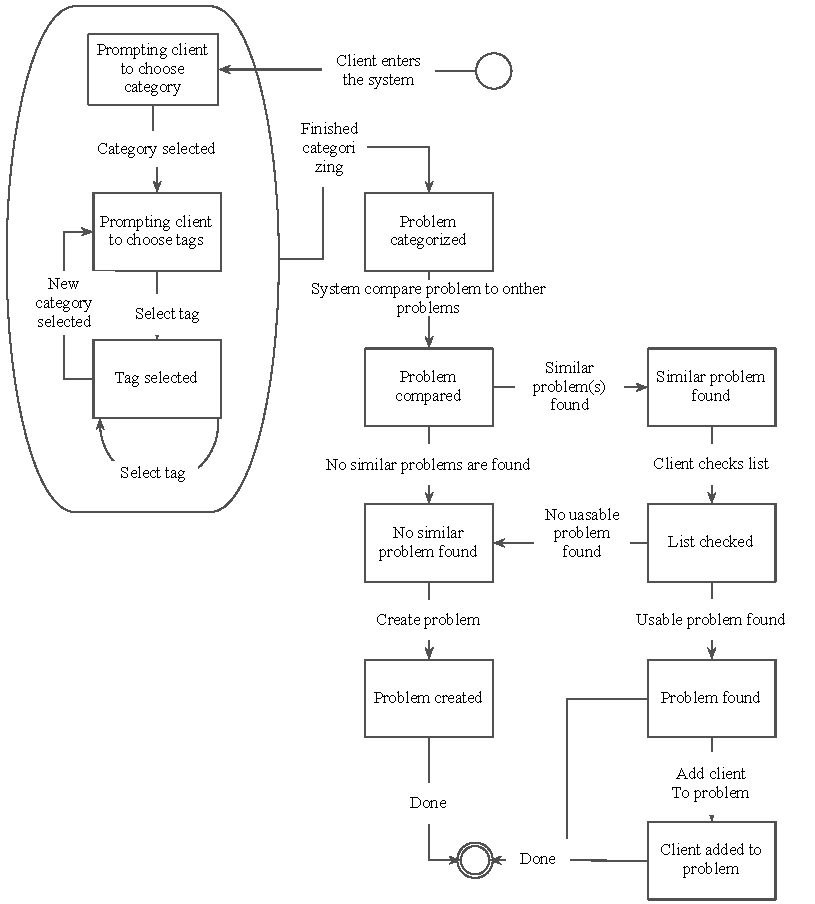
\includegraphics[scale=1]{input/application_domain_analysis/submit_problem_use_case}
\caption{A diagram of the use case \ucsproblem{}. The use case is described in detail in figure \ref{fig:ucsproblem}.}
\label{fig:submit_problem_use_case}
\end{center}
\end{figure}



\paragraph{\ucsolproblem{}} The use case \ucsolproblem{} is the \astaff{}s primary working usage of the system. This is where he goes to get his \todolist{} and to solve problems. The use case is described in figure \ref{fig:ucsolproblem} and a diagram is shown in figure \ref{solve_problem_use_case}.


\begin{sadlist}[h]{\ucsolproblem[c]}{Description of the use case \ucsolproblem{}.}{fig:ucsolproblem}
\sadb{Use Case:} The use case is initialized when the \astaff[] wants to check his \todolist[]. He is then presented with a list of unsolved problems assigned to him. He can then click on one of the problems to solve the problem, see status of it, add comments to it, search the database for similar problem, reassign it or delete it.
\sadb{Objects:} 
\sadb{Functions:}
\end{sadlist}

\begin{figure}[htbp]
\begin{center}
 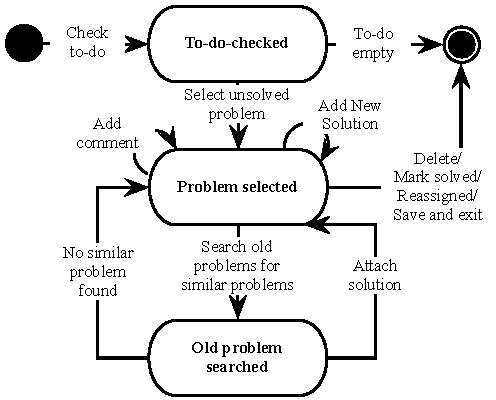
\includegraphics[scale=1]{input/application_domain_analysis/solve_problem_use_case}
\caption{A diagram of the use case \ucsolproblem{}.}
\label{fig:solve_problem_use_case}
\end{center}
\end{figure}

